\subsection{Счётчик с аутентификаций Галуа}
\selectlanguage{russian}

Режим счётчика с аутентификацией Галуа был предложен Девидом МакГрю и Джоном Виега в 2004 году (\langen{Galois/Counter Mode, GCM}, рис.~\ref{fig:GCM}, \cite{McGrew:Viega:2004}). Данный режим обеспечивает одновременно конфиденциальность и целостность, при условии правильного использования.

\begin{figure}[bt]
	\centering
	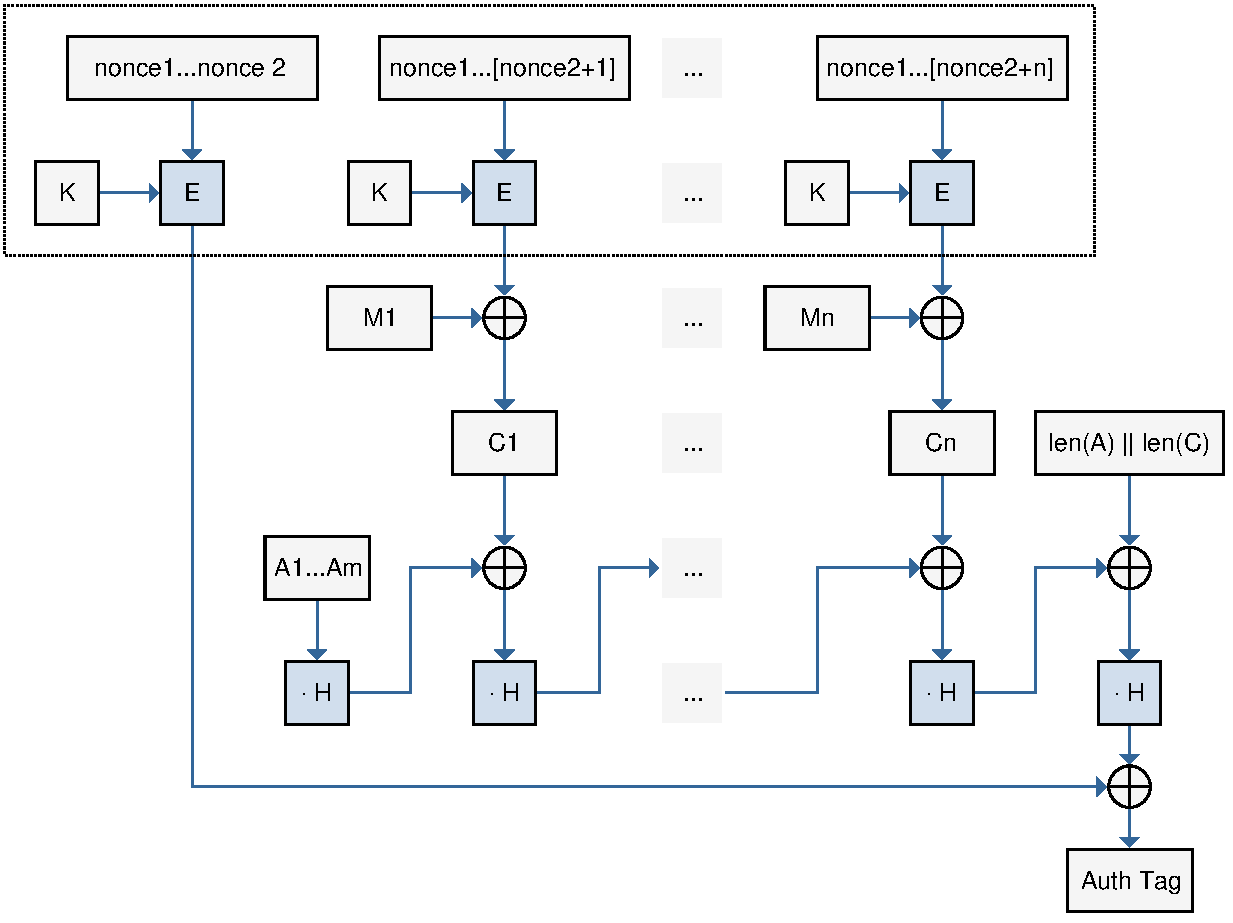
\includegraphics[width=1\textwidth]{pic/GCM}
	\caption{Режим счётчика с аутентификаций Галуа. Пунктирной рамкой выделена область формирования \emph{гаммы}, независящей от открытого текста.}
	\label{fig:GCM}
\end{figure}

Результатом работы режима, кроме набора шифроблоков, является тег аутентификации, который должен быть использован принимающей стороной для проверки целостности сообщения. Как и в режиме выработки имитовставки, генерация данного тега возможна только легальным пользователем -- знающим секретный ключ, который был использован для шифрования данных.

<<Верхняя>> часть режима является режимом работы счётчика. В качестве первого значения берётся дополнение нулями вектора инициализации до размера обрабатываемого блока. Потом, как и в режиме CTR, правая часть увеличивается на 1 для каждого следующего блока. Значения счётчика шифруются на секретном ключе $K$ для получения блоков гаммы. Самый первый блок полученной гаммы используется не для шифрования открытого текста, а для формирования тега аутентификации.

Сам тег аутентификации вырабатывается следующим образом. На вход <<подрежима>> генерации тега сначала (опционально) подаются дополнительные данные (\langen{additional authenticated data, AAD}), которые не нужно шифровать в режиме GCM, но которым нужно обеспечить целостность. Например, это может быть заголовок передаваемого пакета данных. После того, как эти данные закончатся, на вход начнут подаваться блоки шифротекста $C_1, C_2, \dots, C_n$. Использование блоков шифротекста, а не открытого текста, позволяет получателю проверить целостность передаваемых данных до того, как приступит к расшифровке. В качестве последнего блока выступает конкатенация длин дополнительных данных и открытого текста.

Формирование тега происходит через побитовое сложение результата предыдущего блока с новым блоком AAD или $C_j$ и умножение результата на константу $H$, которая в двоичном виде равна результату шифрования нулевого вектора (блока, заполненного нулями) на ключе $K$:

\[ \begin{array}{l}
	H = E_K ( 0^{\{n\}} ) \\
\end{array} \]

Умножение на константу $H$ происходит в поле Галуа $\GF{2^{n}}$. Рекомендуемый порождающий многочлен поля для шифра AES (с размером блока 128 бит):

\[ \begin{array}{l}
	f(x) = x^{128} + x^7 + x^2 + x + 1.
\end{array} \]

Результат умножения самого последнего блока побитово складывается с первым блоком сформированной гаммы.

Данный режим обеспечивает и конфиденциальность, и целостность. Шифровать отдельные блоки можно параллельно, а вычисление тега аутентификации делается намного быстрее, чем шифрование. Однако любая ошибка передачи приведёт к вычислению некорректного тега аутентификации, а отличить изменение текста в результате ошибки передачи от вмешательства злоумышленника принципиально невозможно.